\chapter{Flow and Heat --2D -- Transient -- Rayleigh-Benard instability}

\modinfo{Directory}{RayleighBenardGUI}
\modinfo{Solvers}{\Idx{HeatSolve}, \Idx{FlowSolve}}
\modinfo{Tools}{\Idx{ElmerGUI}}
\modinfo{Dimensions}{2D, Transient}
\modinfo{Author}{Juha Ruokolainen, Peter R{\aa}back}


\subsection*{Case definition}

%\begin{flushleft}
This tutorial is about simulating the developing of the
\Idx{Rayleigh-Benard} instability in a rectangular domain  (Figure
\ref{fg:rb_geometry}) of dimensions 0.01 m height and 0.06 m
length. The simulation is performed with water and the material
parameters of water required by the Elmer model are presented in 
Table \ref{tb:matpar} and can be loaded from the Material Library. 
The temperature difference between the upper and lower boundary is set to
0.5 so that lower one has the temperature of  293.5 K and the upper
one has the temperature of 293 K.


The density of water is inversely proportional to its
temperature. Thus, heated water starts to flow upwards, and colder
downwards due to gravity.  In this case we assume that the
\Idx{Boussinesq} approximation is valid for thermal incompressible
fluid flow. In other words, the density of the term $\rho$$\vec{f}$ in
the incompressible Navier-Stokes equation can be redefined by the
Boussinesq approximation
\begin{displaymath}
\rho = {\rho}_0(1-\beta(T-{T}_0))
\end{displaymath}
where $\beta$ is the heat expansion coefficient and the subscript 0 
refers to a reference state.


\begin{figure}[h]
\centering
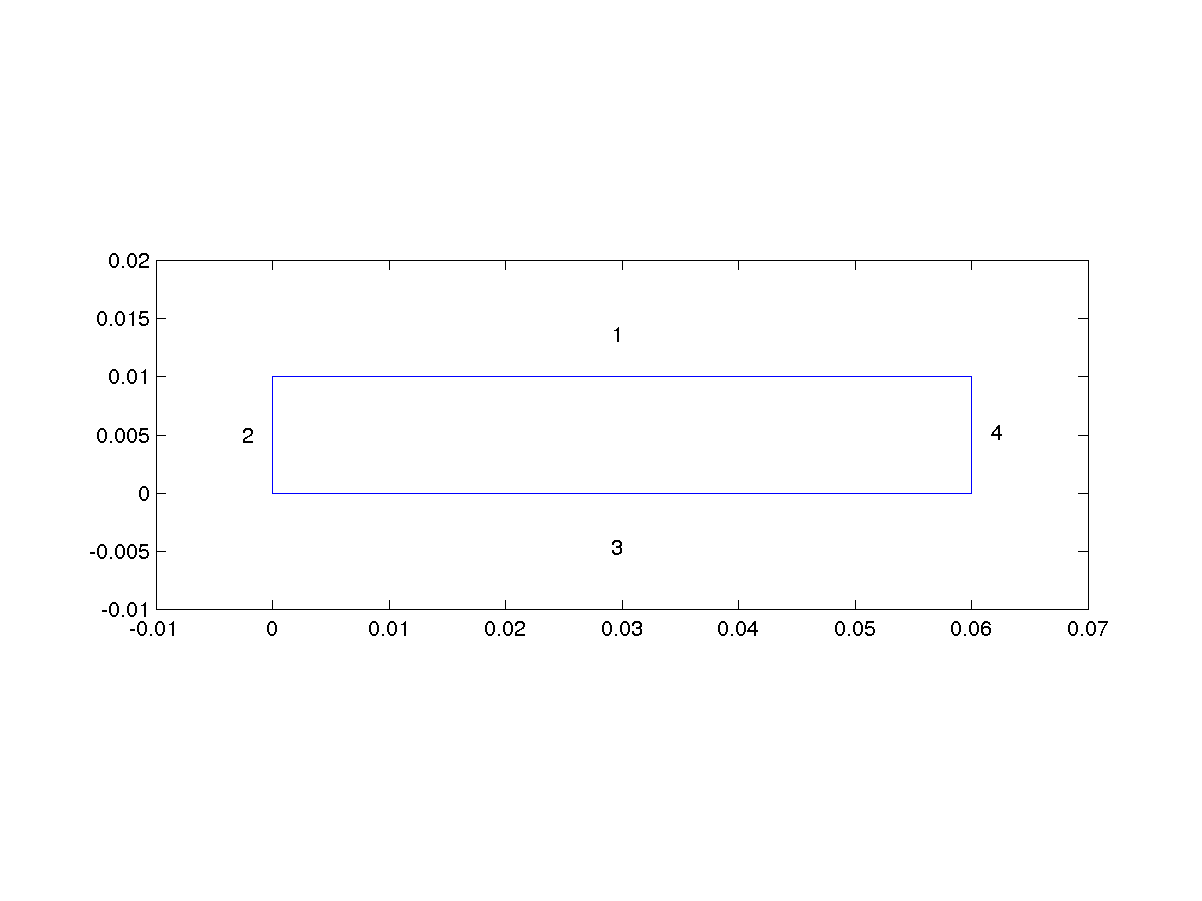
\includegraphics[width=150 mm, height=55 mm]{rb_geometry}
\caption{Domain.}\label{fg:rb_geometry}
\end{figure}  


\begin{table}[h]
\caption{Material parameters for water}
\label{tb:matpar}
\begin{center}
\begin{tabular}{ll} \hline
parameter  & value \\ \hline
density & 998.3 kg/m$^{3}$ \\
viscosity & 1040e-6 Ns/m$^{2}$ \\
heat capacity & 4183 J/(kg$\cdot$K) \\
heat conductivity & 0.58 W/(m$\cdot$K)       \\
heat expansion coefficient & 2.07e-4 K$^{-1}$      \\ 
reference temperature & 293 K       \\ \hline
\end{tabular}
\end{center}
\end{table}


\subsection*{Solution procedure}

The mesh is given in ElmerGrid format in file \texttt{rectangle.grd}, load this file.
\ttbegin
File 
  Open -> rectangle.grd
\ttend
You should obtain your mesh and may check \texttt{Model Summary...} that it consists 
of 3036 bilinear elements.  The geometry and mesh should look like 
figure \ref{fg:rb_geometry}.

There is a possibility to divide and unify edges to simplify the case definition in the future.
\ttbegin
Choose (left wall + right wall (Ctrl down)) -> unify edge
\ttend

After we have the mesh we start to go through the Model menu from the top to bottom. 
In the Setup we choose things related to the whole simulation such as file names, 
time stepping, constants etc.
The simulation is carried out in 2-dimensional Cartesian
coordinates. 2nd order bdf time stepping method is selected with 200 steps
and with step size of two seconds.
Gravity is needed for the buoyancy force and it is defined by a vector with four components. 
The first three components define a unit vector and the fourth its magnitude. 
\ttbegin
Model
  Setup 
    Simulation Type = Transient
    Steady state max. iter = 20
    Time Stepping Method = bdf
    BDF Order = 2
    Time Step Intervals = 200
    Time Step Sizes = 2.0
    Gravity = 0 -1 0 9.82
\ttend
In the equation section we choose the relevant equations and parameters related to their solution. 
In this case we'll have one set of equations (named ``Natural Convection'') which 
consists of the heat equation and of the Navier-Stokes equation.

When defining Equations and Materials it is possible to assign to the bodies immediately, or to use mouse
selection to assign them later. In this case we have just one body and therefore its easier to assign 
the Equation and Material to it directly.
It is important to select the 
convection to be computed since that couples the velocity field to the heat equation.

The system may include non-linear iterations of each equation and steady state iterations 
to obtain convergence of the coupled system. It is often a good idea to keep the number of 
non-linear iterations in a coupled case low. Here we select just one non-linear iteration
for both equations.

For the linear system solvers we are happy to use the defaults. One may however, try out different
preconditioners (ILU1,\ldots) or direct Umfpack solver, for example.
\ttbegin
Model
  Equation
    Name = Natural Convection
    Apply to Bodies = 1
    Heat Equation
      Active = on
      Convection = Computed
      Edit Solver Setting
        Nonlinear System
          Max. iterations = 1
    Navier-Stokes 
      Active = on
      Edit Solver Setting
        Nonlinear System
          Max. iterations = 1
    Add 
    OK
\ttend        
The Material section includes all the material parameters.
They are divided into generic parameters which are direct properties of the material
without making any assumptions on the physical model, such as the mass. Other properties assume
a physical law, such as conductivities and viscosity. 

Here we choose water at room temperature from the Material Library.
You may click through the material parameters of the various solvers to ensure that
the properties are indeed as they should be. Any consistent set of units may be used in Elmer.
The natural choice is of course to perform the computations in SI units. 

Apart from the properties from the material database, we enter a
reference temperature for the Boussinesq approximation.    

\ttbegin
Model
  Material
    Apply to Bodies = 1 
    Material library    
      Water (room temperature)
    General 
      Reference Temperature = 293
    Add
    OK
\ttend

A Body Force represents the right-hand-side of a equation. It is generally 
not a required field for a body. In this case, however, we apply the buoyancy resulting from
heat expansion as a body force to the Navier-Stokes equation.
\ttbegin
Model
  Body Force
    Name = Buoyancy
    Apply to Bodies = 1
    Navier-Stokes
      Boussinesq = on
    Add 
    OK
\ttend    

Initial conditions should be given to transient cases. In this case we choose a 
constant Temperature field and an small initial velocity that initializes the symmetry break. 
\ttbegin
Model
  Initial Condition 
    Name = Initial Guess
    Heat Equation
      Temperature = 293
    Navier-Stokes
      Velocity 1 = 1.0e-9
      Velocity 2 = 0.0
\ttend

Only one boundary condition may be applied to each boundary and therefore all the 
different physical BCs for a boundary should be grouped together. In this case the
Temperature and Velocity. The side walls are assumed to be adiabatic.
\ttbegin
Model
  BoundaryCondition
    Name = Bottom
    Heat Equation
      Temperature = 293.5
    Navier-Stokes 
      Velocity 1 = 0.0
      Velocity 2 = 0.0
    Add
    New

    Name = Top
    Heat Equation
      Temperature = 293
    Navier-Stokes 
      Velocity 1 = 0.0
      Velocity 2 = 0.0
    Add 
    New
 
    Name = Sides
    Navier-Stokes 
      Velocity 1 = 0.0
      Velocity 2 = 0.0
    Add
\ttend   

The conditions may also be assigned to boundaries in the Boundary condition menu, or 
by clicking with the mouse. Here we use the latter approach as that spares us of the 
need to know the indexes of each boundary.
\ttbegin
Model
  Set boundary properties
    Choose Bottom -> set boundary condition Bottom
    Choose Top -> set boundary condition Top
    Choose Sides -> set boundary condition Sides
\ttend

For the execution ElmerSolver needs the mesh files and the command file. 
We have now basically defined all the information for ElmerGUI to write 
the command file. After writing it we may also visually inspect the command file.
\ttbegin
Sif 
  Generate
  Edit -> look how your command file came out  
\ttend

Before we can execute the solver we should save the files in a directory. 
The ElmerGUI project includes all the files needed to restart the case.
\ttbegin
File 
  Save Project
\ttend

After we have successfully saved the files we may start the solver
\ttbegin
Run
  Start solver
\ttend
A convergence view automatically pops up showing relative changes of each iteration.

When there are some results to view we may start the postprocessor also
\ttbegin
Run
  Start ParaView
\ttend


\subsection*{Results}

Due to the number of the time steps the simulation may take around ten minutes.
You may inspect the results with Paraview as the time steps are computed, or
wait until all time steps have been computed. You must reload the files if their number has changed. 
The time series can be automatically animated and even saved to an animation file.

In Figures \ref{fg:rb_temp}  through \ref{fg:rb_velo} the obtained temperature 
and  velocity distribution are presented.  The maximum velocity in the system 
should be about 0.516~mm/s. 

\begin{figure}[h]
\centering
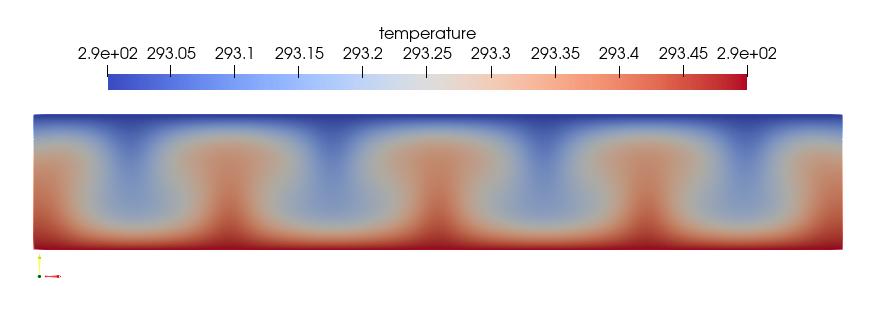
\includegraphics[width=150mm]{rb_temp}
\caption{Temperature distribution}\label{fg:rb_temp}
\end{figure} 

\begin{figure}[h]
\centering
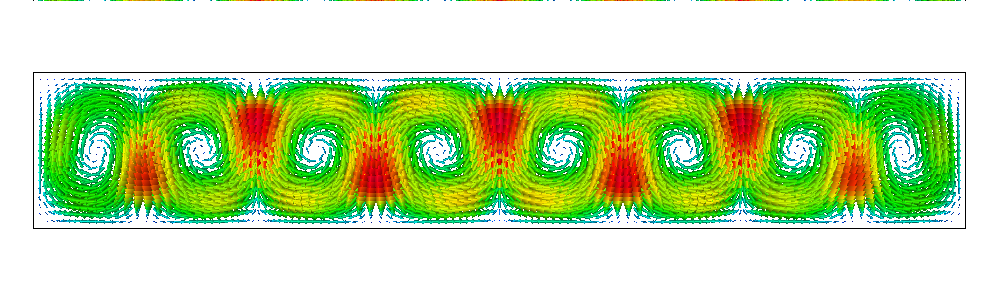
\includegraphics[width=150mm]{rb_velo}
\caption{Velocity magnitudes}\label{fg:rb_velo}
\end{figure} 


\newpage

\subsection*{Extra task: Sensitivity to temperature difference}

If you have time you may try to solve the case with different parameters. Changing the temperature difference
is one way of affecting the instability of the system. Decreasing the temperature differences the system eventually becomes 
steady state and the convection rolls vanish altogether. Increasing the temperature difference may increase the 
number of convection rolls and eventually the system becomes fully chaotic. 
Note that changing the temperature difference also affects to the time scale of the wake. 

\hfill
